\documentclass[10pt]{article}
\usepackage{fontspec}
\setmainfont{Times New Roman}
\setmonofont[Scale=0.85]{Menlo}
\usepackage[russian]{babel}
\usepackage{amsmath}
\usepackage[a4paper,landscape,margin=1.3cm]{geometry}
\usepackage{graphicx,xcolor,colortbl,array,enumitem}
\arrayrulecolor[HTML]{B5B4AB}\definecolor{head}{HTML}{F0EFEC}
\setlist{nosep,leftmargin=1.3em,itemsep=0.25em}
\setlength{\parindent}{0pt}\setlength{\parskip}{0.45em}
\setlength{\tabcolsep}{3.2pt}\renewcommand{\arraystretch}{1.08}
\definecolor{ink2}{HTML}{52514E}
\begin{document}
\selectlanguage{russian}
{\LARGE\bfseries Головы внимания MNN-Pocket-0.3B: главное, графики и механизм}\\[0.2em]
{\color{ink2} 28 слоёв $\times$ 14 голов $=$ 392 голов. Головы делят ключи и значения: групп 2, по 7 в каждой. Текст для проверки: 8192 токенов теста WikiText-2 (окна по 512 токенов).}

\section*{1. Главное}
\begin{itemize}
\item \textbf{Большинство голов смотрит по расстоянию, а не по смыслу.} Из 392 голов 233 смотрят на заданное расстояние (сам токен, предыдущий, окно), 132 усредняют дальний контекст и только 27 выбирают токены по содержанию.
\item \textbf{Быстрые частоты RoPE кодируют расстояние, медленные~— содержание.} «Предыдущий токен» берёт 0,44 преимущества цели на частотах с периодом меньше 20 токенов. «Тот же токен», индукция и сток берут 0,85, 0,92 и 0,69 на частотах с периодом больше 20 тысяч токенов.
\item \textbf{Спад с расстоянием задаёт один вес нормализации.} Частота $m{=}17$ (период 9676 токенов) главная у 218 голов; её усиливает вес нормализации ключей (до 12,1 при медиане 2,1). Если в слое 0 заменить его на медиану, все 14 голов начинают смотреть далеко: доля внимания дальше 256 токенов растёт с 0,30 до 0,63 в среднем.
\item \textbf{«Предыдущий токен» держится на быстрых частотах на любой глубине.} Таких голов 10 (слои 0, 2, 4, 9, 13, 16, 19, 27), у 9 из них частоты с периодом меньше 20 токенов дают не меньше четверти преимущества цели; у 10 самая быстрая частота сдвинута ровно на один токен.
\item \textbf{Сток создают отдельные нейроны MLP.} Один нейрон MLP слоя 6 (номер 2173) на позиции 0 срабатывает в 3351 раз сильнее обычного и даёт 0,99 записи MLP в этой позиции. Норма остаточного потока там становится в 50 раз больше, чем на других позициях. Сток заметен со слоя 6, приписку «+ сток» имеют 147 голов из 392; в слоях 18–27 на первый токен уходит 0,18–0,32 внимания.
\item \textbf{Индукция собрана из двух голов.} Ключ индукционной головы целиком приходит из предыдущих голов (у 5 из 6 главный источник~— голова «Предыдущий токен»), запрос~— сам текущий токен.
\item \textbf{Чем глубже, тем меньше решает сам токен.} Он объясняет 1,00 запроса в слое 0, 0,60 в слое 5 и 0,30–0,43 после слоя 12.
\item \textbf{Главную частоту запроса питают сначала MLP, потом головы.} В слоях 1–15 до 0,82 главной частоты приходит из MLP предыдущих слоёв, в последних слоях до 0,79~— из голов внимания.
\end{itemize}
\section*{2. Графики}
\noindent\begin{minipage}{\linewidth}
\textbf{Рисунок 1.} Сверху~— куда в среднем уходит внимание голов слоя; снизу~— сколько голов каждого вида в слое.
\begin{center}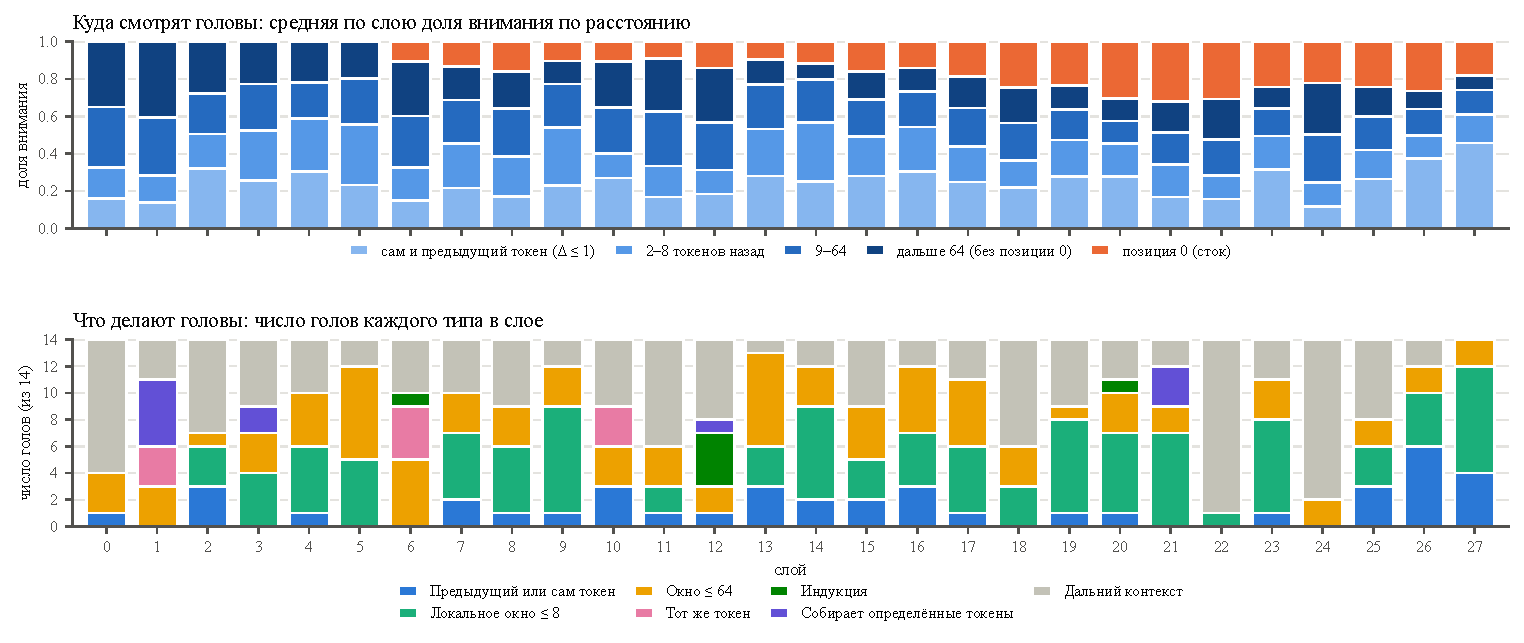
\includegraphics[width=0.76\linewidth]{heads_pocket03b_fig1.pdf}\end{center}
\end{minipage}
\par
\noindent\begin{minipage}{\linewidth}
\textbf{Рисунок 2.} Средние по головам слоя: спад с расстоянием, доля запроса и ключа от токена, источники главной частоты, разброс слагаемых логита, веса нормализации, число ключей.
\begin{center}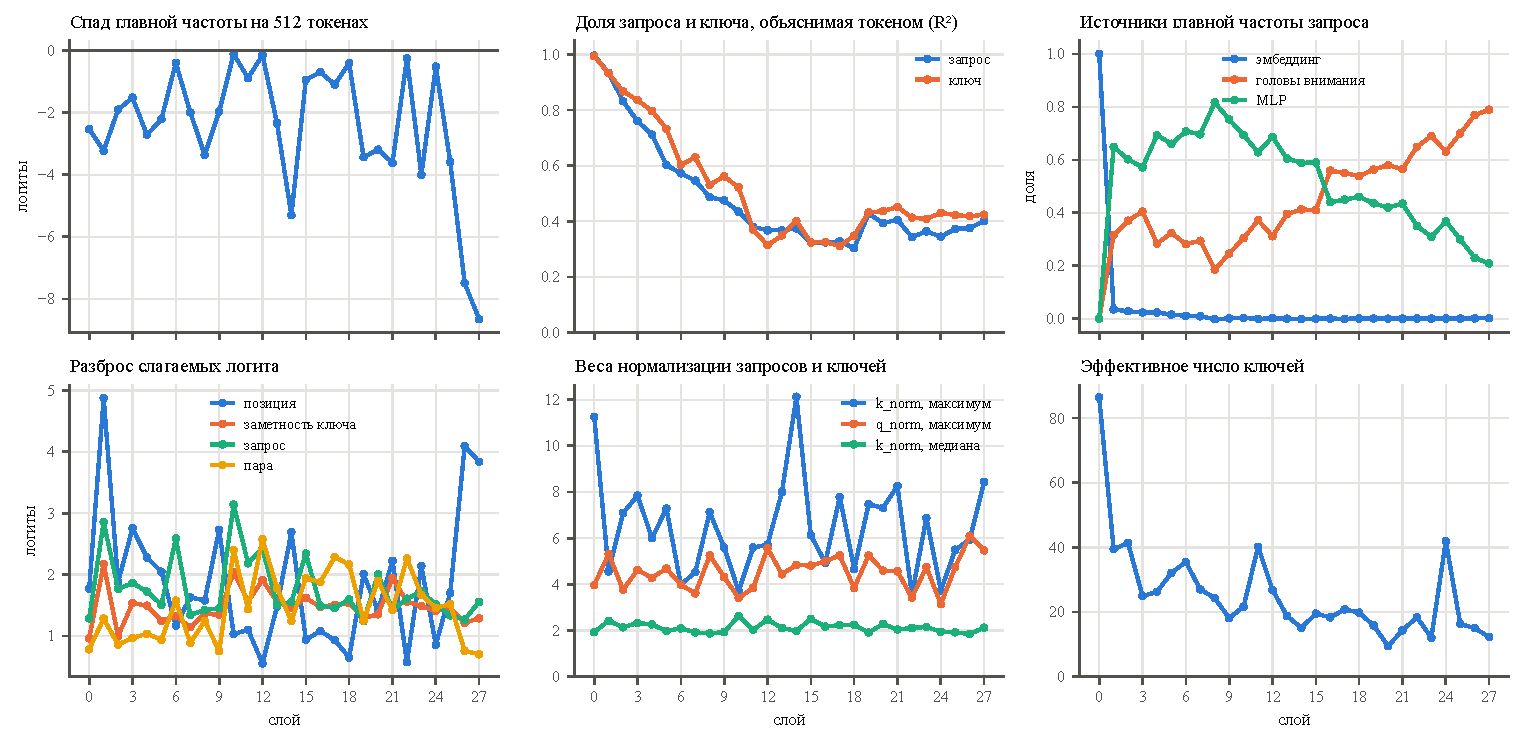
\includegraphics[width=0.78\linewidth]{heads_pocket03b_fig2.pdf}\end{center}
\end{minipage}
\par
\section*{3. Механизм в весах}
\noindent\begin{minipage}{\linewidth}
\textbf{Спад с расстоянием~— одна пара весов нормализации.} В слое 0 вес k\_norm на компоненте 17 равен 11,2, вес q\_norm на компоненте 49~— 4,0; медиана остальных 1,9. Это косинусная часть ключа и синусная часть запроса одной частоты $m{=}17$. Их произведение даёт вклад в логит $-A\sin(\theta_m\Delta)$: почти линейный спад с расстоянием $\Delta$. У голов отличается только сила $A$. Ниже~— что происходит с головами слоя 0, если вес k\_norm заменить на медиану (запросы с контекстом 1024–2048 токенов).
\begin{center}\begin{tabular}{|l|r|r|r|r|r|r|r|r|r|r|r|r|r|r|}\hline \rowcolor{head}\textbf{Голова} & \textbf{0} & \textbf{1} & \textbf{2} & \textbf{3} & \textbf{4} & \textbf{5} & \textbf{6} & \textbf{7} & \textbf{8} & \textbf{9} & \textbf{10} & \textbf{11} & \textbf{12} & \textbf{13} \\ \hline
Дальше 256 токенов, исходные веса & 0,44 & 0,23 & 0,03 & 0,44 & 0,11 & 0,08 & 0,65 & 0,29 & 0,37 & 0,29 & 0,32 & 0,16 & 0,39 & 0,45 \\ \hline
Дальше 256 токенов, вес заменён & 0,66 & 0,53 & 0,38 & 0,75 & 0,40 & 0,43 & 0,80 & 0,75 & 0,70 & 0,67 & 0,64 & 0,63 & 0,76 & 0,69 \\ \hline
Среднее расстояние, исходные веса & 372 & 202 & 22 & 378 & 101 & 79 & 550 & 228 & 305 & 216 & 259 & 139 & 333 & 372 \\ \hline
Среднее расстояние, вес заменён & 638 & 504 & 379 & 759 & 418 & 381 & 757 & 654 & 648 & 550 & 569 & 590 & 746 & 630 \\ \hline\end{tabular}\end{center}
\end{minipage}
\par
\noindent\begin{minipage}{\linewidth}
\textbf{Какие частоты несут выбор.} Логит~— сумма по частотам RoPE, поэтому преимущество цели точно делится между частотами. Быстрые частоты поворачиваются на длине нескольких токенов и различают расстояние; медленные на длине контекста почти не поворачиваются и сравнивают содержание.
\begin{center}{\small\begin{tabular}{|l|r|r|r|r|r|}\hline
\rowcolor{head}\textbf{Вид головы} & \textbf{Голов} & \textbf{Преим., логиты} & \textbf{Период $<$ 20 токенов} & \textbf{20–20 000} & \textbf{$>$ 20 000 токенов} \\ \hline
Предыдущий токен & 10 & $+$11,7 & 0,44 & 0,54 & 0,02 \\ \hline
Сам токен & 31 & $+$10,4 & 0,11 & 0,43 & 0,46 \\ \hline
Тот же токен & 10 & $+$6,6 & 0,00 & 0,15 & 0,85 \\ \hline
Индукция & 6 & $+$6,5 & 0,00 & 0,08 & 0,92 \\ \hline
Приписка «+ сток» & 147 & $+$0,9 & 0,00 & 0,31 & 0,69 \\ \hline
\hline\end{tabular}}\end{center}
\end{minipage}
\par
\noindent\begin{minipage}{\linewidth}
\textbf{Откуда берётся выбор головы.} Логит линеен и по запросу, и по ключу, а оба точно раскладываются по источникам остаточного потока. Поэтому преимущество цели над остальными токенами (в логитах) делится между источниками без приближений (ошибка суммы 9$\cdot 10^{-6}$ логита).
\begin{center}{\small\begin{tabular}{|l|p{3.7cm}|r|r|c|c|c|p{3.5cm}|}\hline
\rowcolor{head}\textbf{Вид головы} & \textbf{Цель} & \textbf{Голов} & \textbf{Преим., логиты} & \textbf{Ключ: эмб. / головы / MLP} & \textbf{Запрос: эмб. / головы / MLP} & \textbf{Косинус: своя / чужая} & \textbf{Главный источник ключа} \\ \hline
Предыдущий токен & токен перед текущим & 10 & $+$11,7 & 0,11 / 0,41 / 0,48 & 0,12 / 0,40 / 0,48 & 0,24 / 0,23 & MLP0 (4 гол.), MLP8 (4 гол.) \\ \hline
Сам токен & текущий токен & 31 & $+$10,4 & 0,00 / 0,65 / 0,34 & 0,00 / 0,64 / 0,36 & 0,35 / 0,24 & MLP8 (8 гол.), L13.H7 (3 гол.) \\ \hline
Тот же токен & прошлые вхождения того же токена & 10 & $+$6,6 & 0,07 / 0,34 / 0,59 & 0,07 / 0,22 / 0,70 & 0,59 / 0,37 & MLP0 (7 гол.), MLP8 (3 гол.) \\ \hline
Индукция & токен после прошлого вхождения текущего & 6 & $+$6,5 & 0,00 / 1,00 / 0,01 & 0,01 / 0,35 / 0,64 & 0,48 / 0,31 & L9.H5 (4 гол.), L5.H6 (1 гол.) \\ \hline
Приписка «+ сток» & первый токен текста & 147 & $+$0,9 & 0,00 / -1,91 / 2,91 & 0,00 / 0,32 / 0,68 & 0,34 / 0,26 & MLP6 (145 гол.), MLP5 (2 гол.) \\ \hline
\hline\end{tabular}}\end{center}
«Косинус»~— между запросом и ключом одной позиции и разных позиций. У стока доли выходят за пределы 0–1: MLP создают ключ первого токена, а предыдущие головы частично его гасят.
\end{minipage}
\par
\begin{itemize}
\item \textbf{Индукция.} Ключ целиком приходит из предыдущих голов, главным образом из голов «Предыдущий токен» (12.0 ← 9.5 (0,45), 12.1 ← 9.5 (0,43), 12.3 ← 9.5 (0,46), 12.4 ← 9.5 (0,44)): они записывают в позицию, какой токен стоял перед ней. Запрос несёт сам текущий токен (эмбеддинг / головы / MLP: 0,01 / 0,35 / 0,64). Совпадение даёт цели $+$6,5 логита.
\item \textbf{Сам токен.} У 24 из 31 таких голов пик позиционного ядра приходится на $\Delta{=}0$: быстрые частоты стоят без сдвига и дают 0,11 преимущества цели. Кроме того, запрос и ключ читают одни и те же направления остаточного потока: косинус между ними 0,35 на своей позиции против 0,24 на чужой. Цель получает в среднем $+$10,4 логита. Источники у запроса и ключа одни и те же: в среднем 3,3 из 5 главных совпадают.
\item \textbf{Тот же токен.} Запрос и ключ собраны из одних и тех же источников, которые несут сам токен (эмбеддинг / головы / MLP: 0,07 / 0,22 / 0,70 у запроса и 0,07 / 0,34 / 0,59 у ключа). У одинаковых токенов они совпадают; совпадение идёт по медленным частотам (0,85 преимущества), поэтому не зависит от расстояния. Прошлое вхождение получает $+$6,6 логита.
\item \textbf{Сток.} Один нейрон MLP слоя 6 (номер 2173) на позиции 0 срабатывает в 3351 раз сильнее обычного и даёт 0,99 записи MLP в этой позиции. Норма остаточного потока на позиции 0 вырастает с 1,4 до 49,9 от обычной, 0,65 энергии в координатах 358, 620, 75, 578. Проекция ключей читает этот вектор на медленных частотах (0,69 преимущества): у 145 из 147 голов со стоком главный источник ключа позиции 0~— MLP слоя 6. Постоянный вектор MLP слоя 0, наоборот, пишут многие нейроны: на 90\,\% записи нужно 471 из 2560.
\end{itemize}
\begin{itemize}
\item \textbf{Предыдущий токен.} Быстрые частоты RoPE поворачиваются на заметный угол за один токен (самая быстрая~— на 1 радиан). Фазы запроса и ключа сдвинуты так, что пик приходится на $\Delta{=}1$. Частоты с периодом меньше 20 токенов дают 0,44 преимущества цели.
\item \textbf{Спад в следующих слоях включает MLP.} В слое 1 от 0,59 до 0,68 главной частоты запроса приходит из MLP слоя 0: MLP пишет в остаточный поток постоянный вектор, а проекции следующего слоя читают его на этой частоте.
\item \textbf{Головы с общими ключами делают похожую работу.} В слое 1 одна группа собирает служебные слова, другая ищет тот же токен; в слое 2 одна группа позиционная, другая смотрит далеко.
\end{itemize}
\section*{4. Как получены результаты}
Логит внимания любой головы точно равен сумме по частотам RoPE:
\[ s_h(i,j) \;=\; \frac{1}{\sqrt{D}}\,\mathrm{Re}\sum_{m} z^{q}_{h,m}(i)\,\overline{z^{k}_{g,m}(j)}\,e^{\,i\theta_m (i-j)}, \qquad \theta_m = 10^{-12m/D}, \]
где $z^q$, $z^k$~— запрос и ключ после нормализации (QK-norm), записанные комплексными числами по частотам ($m$-я частота~— компоненты $m$ и $m+D/2$), $\Delta=i-j$~— расстояние между токенами. В слое 0 запрос и ключ зависят только от токена, дальше~— от контекста, поэтому берутся из прогона текста.
\begin{itemize}
\item \textbf{Внимание пересчитано по этой формуле} и совпадает с выходом модели: относительная ошибка не больше $8\cdot 10^{-6}$.
\item \textbf{Источники запроса и ключа найдены точно.} Вход слоя~— сумма эмбеддинга и записей всех предыдущих голов и MLP в остаточный поток. Нормализация и проекции линейны с точностью до одного множителя на позицию, поэтому каждая компонента запроса и ключа раскладывается по источникам без приближений (ошибка суммы не больше $2\cdot 10^{-6}$).
\item \textbf{Позиционное ядро} головы~— логит при средних запросе и ключе как функция расстояния. Оно показывает, как голова смотрит на расстояние независимо от токенов, и раскладывается по частотам: у каждой частоты амплитуда и сдвиг пика.
\end{itemize}
\textbf{Границы отчёта.} Виды голов определены по порогам на одном корпусе (WikiText-2, 8192 токенов). Разложение по источникам объясняет, откуда берутся запрос и ключ, то есть куда голова смотрит; что она после этого записывает в остаточный поток, в отчёт не входит.
\end{document}
